
\section{\rnn{} Aggreament}%
\label{sec:off_ana}

This section is dedicated to a more detailed assessments of the \rnn{} behavior 
in the period 2017-2018 with respect to the previous electron trigger cut-based strategy.
Using \Zee{} \tnp{} selection, the agreement between the two triggers and
possible biases, caused by the introduction of the \rnn{} using the variables
employed by the likelihood algorithm, were investigated.
Since offline and final HLT electron
selections are based on such variables, limiting the evaluation to them suffices
to understand any possible impact of the \rnn{} algorithm in most analyses.
Additionally, these variables are interesting since they compact the input space
in a set of few variables with low correlation and high interpretability power. 
%One should keep in mind that the \rnn{} algorithm had access only to the ring description during Run~2 operation.

As indicated in Table~\ref{tab:quadrant_vs_agreement}, two analyses were performed to assess the
trigger performance with and without \rnn{}, when applied to the tag (Agreement Analysis) and
to the probe (Quadrant Analysis). The Tag \& Probe events have one probe electron that was not 
used to decide the selection of that event at the trigger level.


\begin{table}[ht!]\footnotesize
\centering
\caption{Customized \Zee{} \tap{} selection criteria employed in the
agreement and quadrant analyses in 2017-2018 period}.%
\label{tab:quadrant_vs_agreement}
\resizebox{\textwidth}{!}{%
  \begin{tabular}{p{2cm}p{4.5cm}p{5.5cm}}
\hline
\hline
\hline
& Agreement Analysis (Section~\ref{ssec:agreement}) & Quadrant Analysis
(Section~\ref{ssec:quadrant}) \\
\hline
\hline
tag (and event) & trigger selection comparison & primary lowest unprescaled electron triggers \\
\hline
probe & \vloose & trigger selection comparison with offline selection fixed to
the same trigger requirement \\
\hline
\hline
\hline
\end{tabular}
}
\end{table}

The Quadrant Analysis allows to directly assess possible bias caused by the
introduction of the \rnn{} by comparing the profiles for all possible disjoint
decisions from the two trigger classifiers. Hence, it is possible for the classifiers
to agree by both accepting or rejecting the event. Likewise, they are able to
disagree in two possible cases where either one decides to accept the event
while the other rejects it.

Although it is reasonable to expect that the shower development of the tag and
the probe are independent from each other, and that the \rnn{} when applied to
the tag selection cannot, in principle, alter the profile of the probes besides
changing the number of \tnp{} pairs. Such evaluation of any possible systematic effect caused by the introduction of the \rnn{} in the extraction of the likelihood PDFs, employed for offline and final HLT selection, is performed by the Agreement Analysis.



\subsection{Quadrant Analysis}\label{ssec:quadrant}

The Quadrant Analysis was developed to compare the decision of two classifiers. Given signal candidates and two classifiers, these are the possibilities: either both accept or reject the candidates or only one accepts the candidates. The four possible decision quadrants are evaluated from shower shape distributions. Furthermore, in this analysis, it's also possible to compare the disagreement between two classifiers. The disagreement between two classifiers $\textbf{A}$ and $\textbf{B}$ can be defined as:

\begin{equation}
    \text{disagreement} = \frac{N_{\textbf{A}}+N_{\textbf{B}}}{N_{\textbf{A}}+N_{\textbf{B}}+N_{\textbf{AB}}+N_{!\textbf{AB}}}
    \label{eq:disagreement}
\end{equation}
where $N_{\textbf{A}}$ ($N_{\textbf{B}}$) is the total of candidates accepted exclusively by classifier $\textbf{A}$ ($\textbf{B}$) and $N_{\textbf{AB}}$ ($N_{\textbf{!AB}}$) is the total of candidates accepted (rejected) by both classifiers.

In this approach, only collision data collected by the primary triggers with an equivalent offline selection are considered\footnote{I.e., if a \tight{} trigger leg is being evaluated, it also applied the \tight{} offline selection to the candidate.}.
Results in Section~\ref{top:quadrant_results} show
trigger selection performance using \tight{} requirement for the duplicated triggers during 2017.

\subsubsection{Results}\label{top:quadrant_results}



The Quadrant Analysis starts with the variable \reta{} for being one of the best electron-jet discriminant variables employed in the likelihood
algorithm~\cite{aaboud2019electron}. 



As shown in Figure~\ref{fig:quadrant_calo_variables_30GeV_eta}, the disagreement is small and bounded for most cases at the 1\% level for the coverage of all calorimetry variables. 
This behavior is also observed for \et{} slices. 
One should note that the working points of both triggers are not exactly the same, although the \rnn{} aims at keeping the same signal efficiency as the cut-based strategy and was operating as desired.  
%Thus, much of the differences reflect this difficulty. 
In other words, 
%One should note that the integral of the single trigger cases is related to the limitation in the precision of setting the working point of both triggers to be exactly the same. In other words, 
the difference in height of the blue and red profiles in Figure~\ref{fig:quadrant_calo_variables_30GeV_eta} is mainly due to the small differences in efficiencies between the two triggers.
From the operation, it was realized that such working point matching was better in the $0.6<\abseta{}<0.8$ region. Hence, comparison between profiles is simpler to be performed there.
%Hence, comparison between profiles is simpler to be performed in the $0.6<\abseta{}<0.8$, which exhibits very similar performance.

For all variables in this region, both triggers behave very similarly (see Figure~\ref{fig:quadrant_calo_variables_30GeV}), even if some slight shifts can be observed in few profiles. This is the case of \reta{} and \rphi{}, where the \rnn{} trigger is consistently collecting slightly more events in the signal region, i.e. respectively with slight tighter showers in $\eta{}$ and $\phi{}$ in the EM2. The \rnn{} trigger behavior shows an even lower effect in the \rhad{}, where tighter tails are observed, resulting in fewer electrons with 10\% to 30\% energy in EM1, 1\% to 2\% in EM3 and more than 4 GeV hadronic leakage. \eratio{} also shows a slightly bias towards collecting more events in the signal region with the \rnn{} trigger. Interestingly, a few events are accepted by the trigger with \rnn{}, when $0.5<\eratio{}<0.7$, probably due to electrons resulting from premature showers with barycenter near the edge of two strips

\begin{figure}[h!]
\centering
\begin{subfigure}[c]{.49\textwidth}
\centering
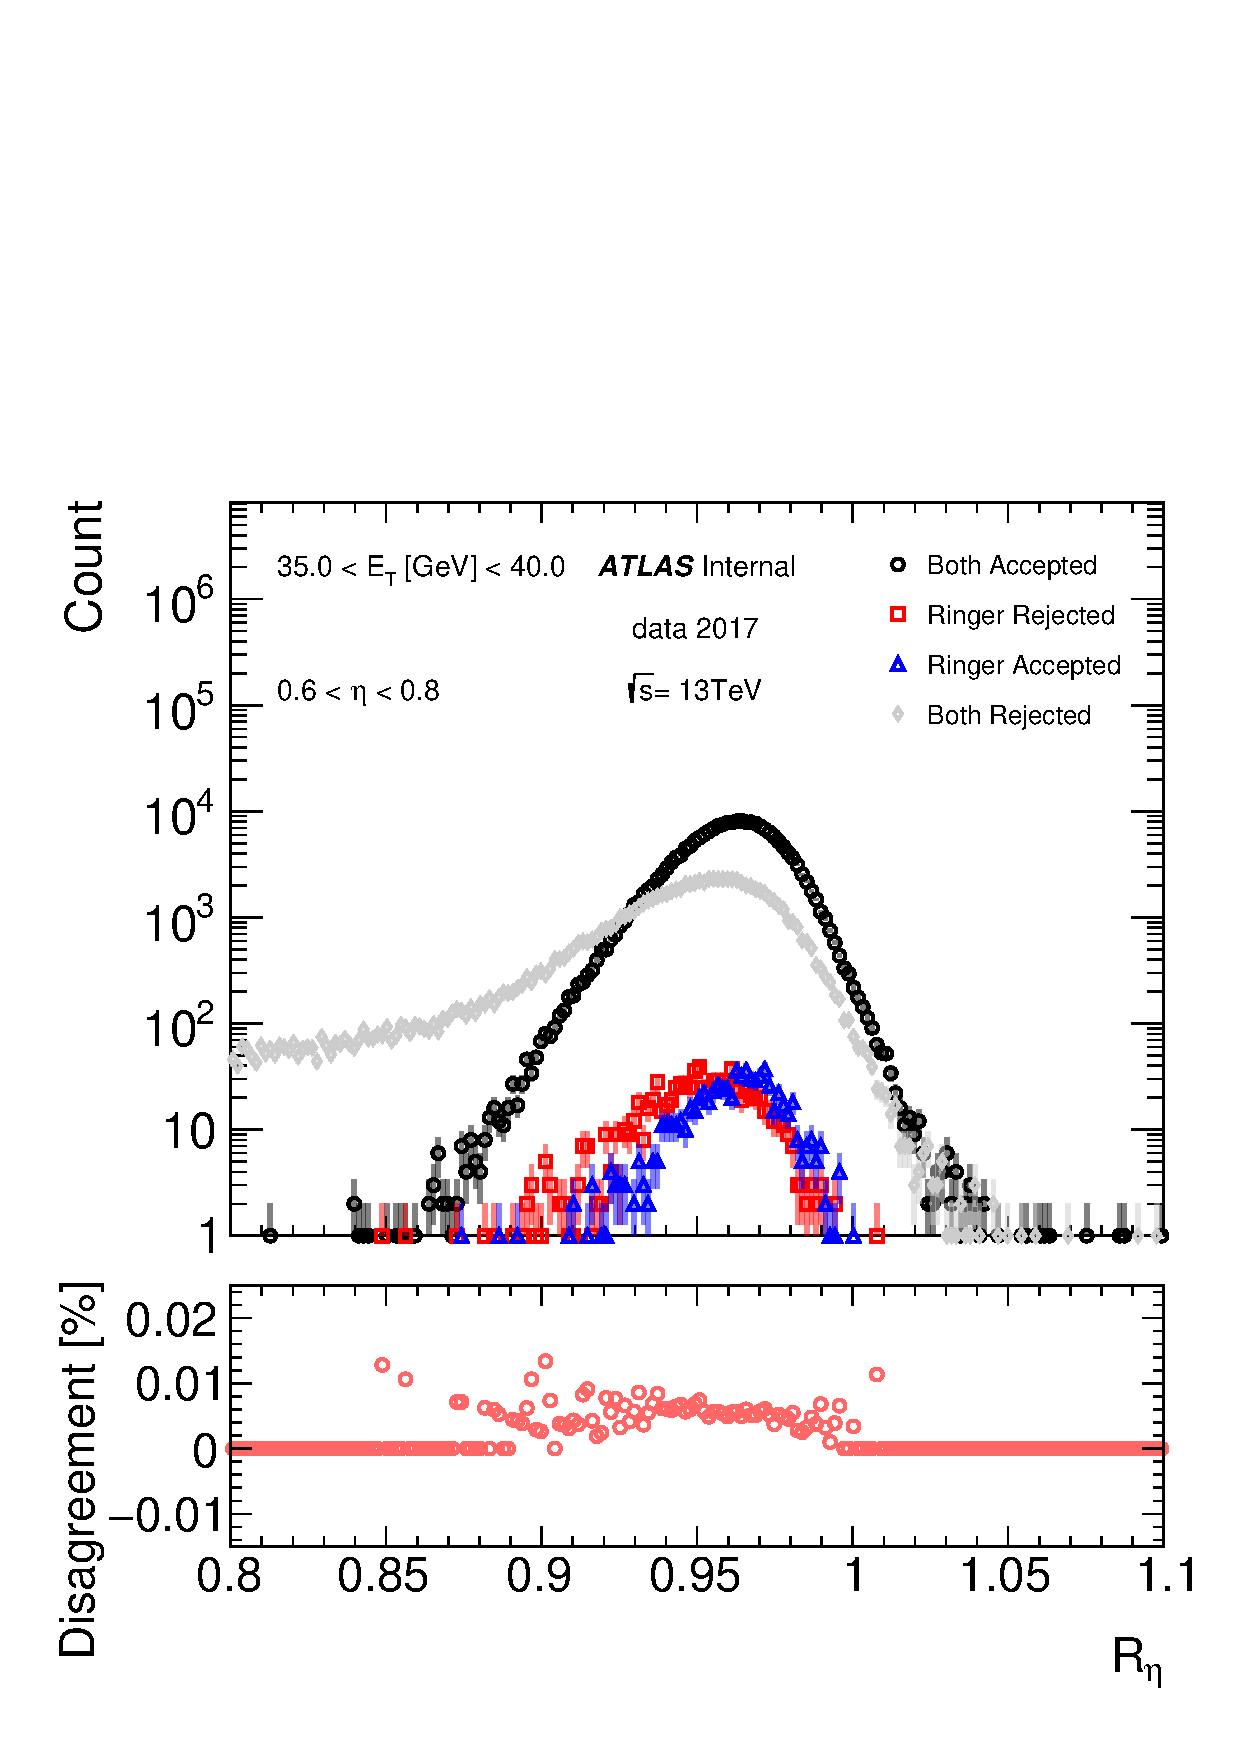
\includegraphics[width=\textwidth]{sections/04_analysis/figures/quadrant_plots/reta.pdf}
\caption{}
\label{fig:quadrant_calo_variables_30GeV_eta}
\end{subfigure}
%\hfill
\begin{subfigure}[c]{.49\textwidth}
\centering
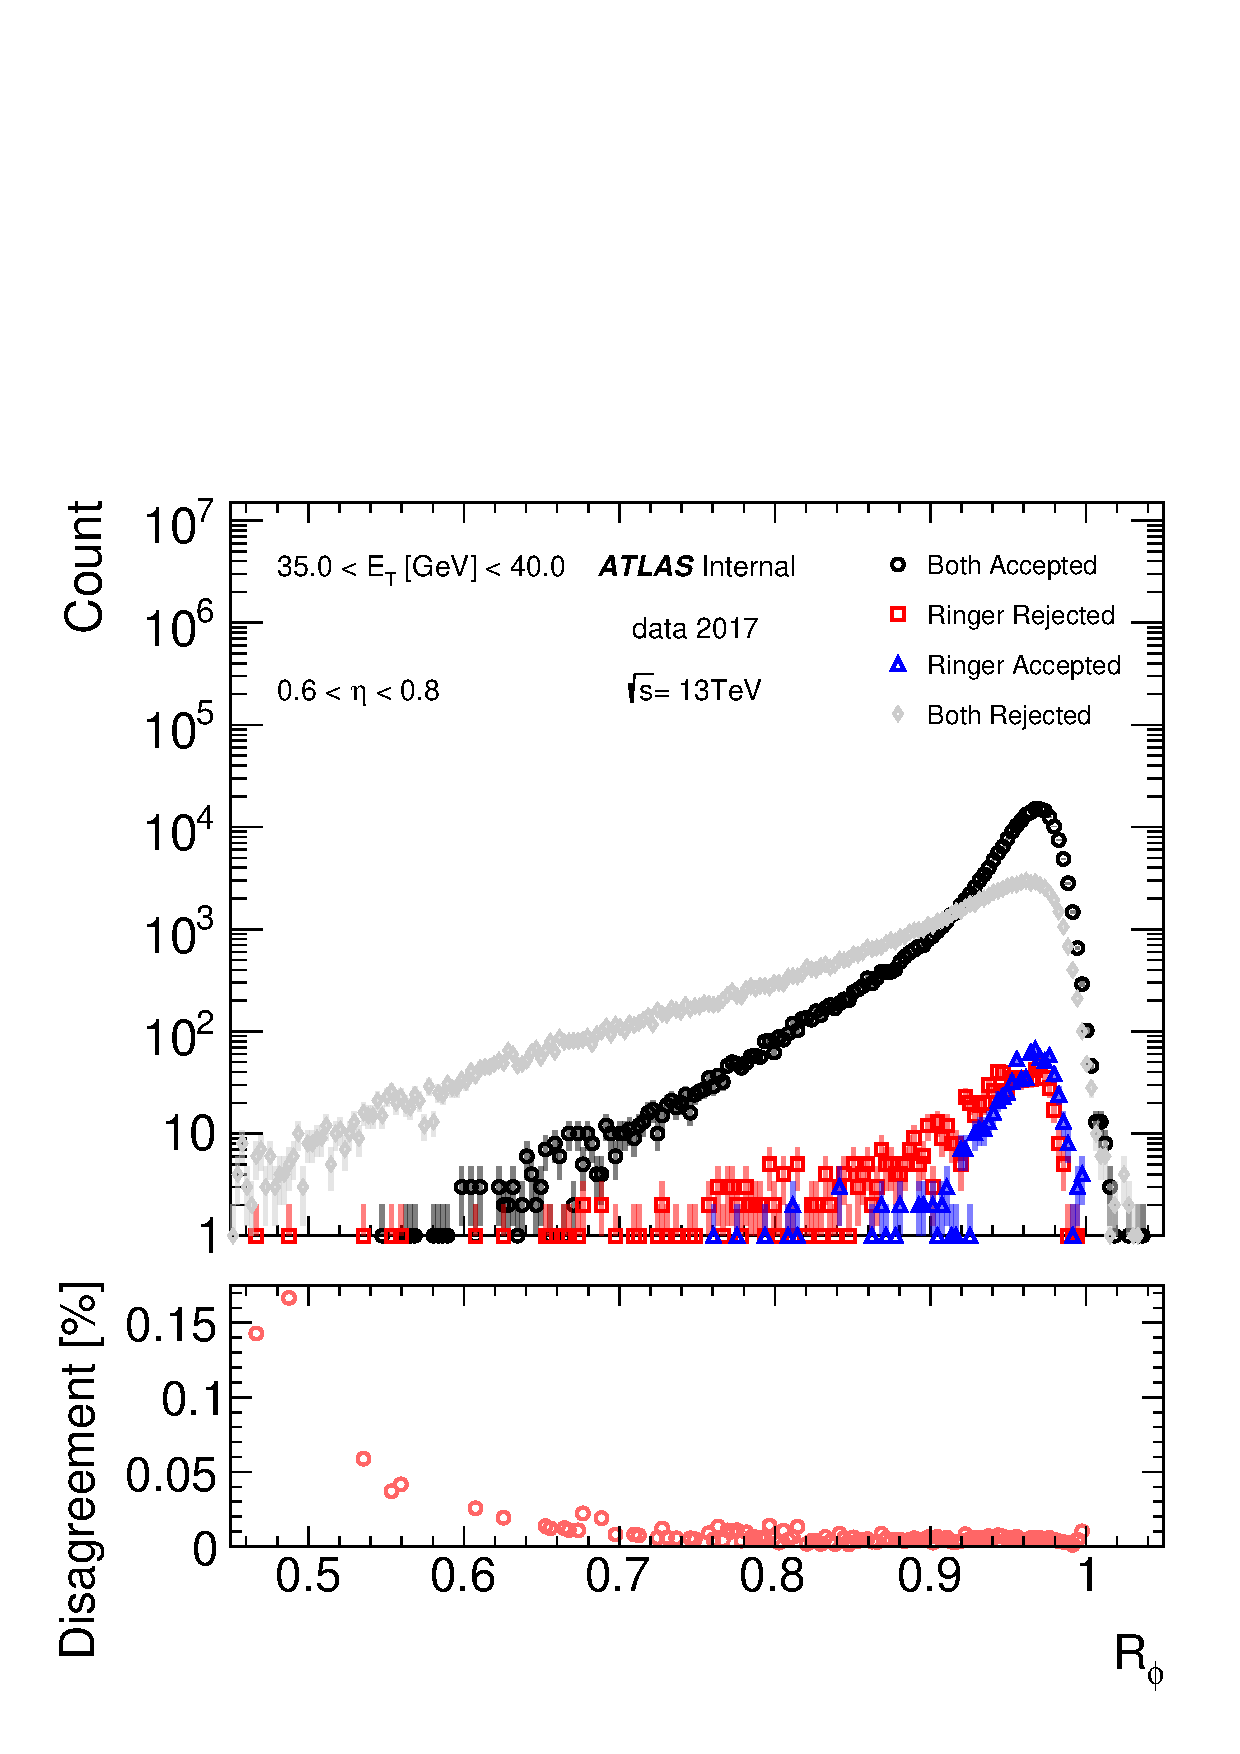
\includegraphics[width=\textwidth]{sections/04_analysis/figures/quadrant_plots/rphi.pdf}
\caption{}
\end{subfigure} 
%\end{figure}
%\begin{figure}[p]\ContinuedFloat
\begin{subfigure}[c]{.49\textwidth}
\centering
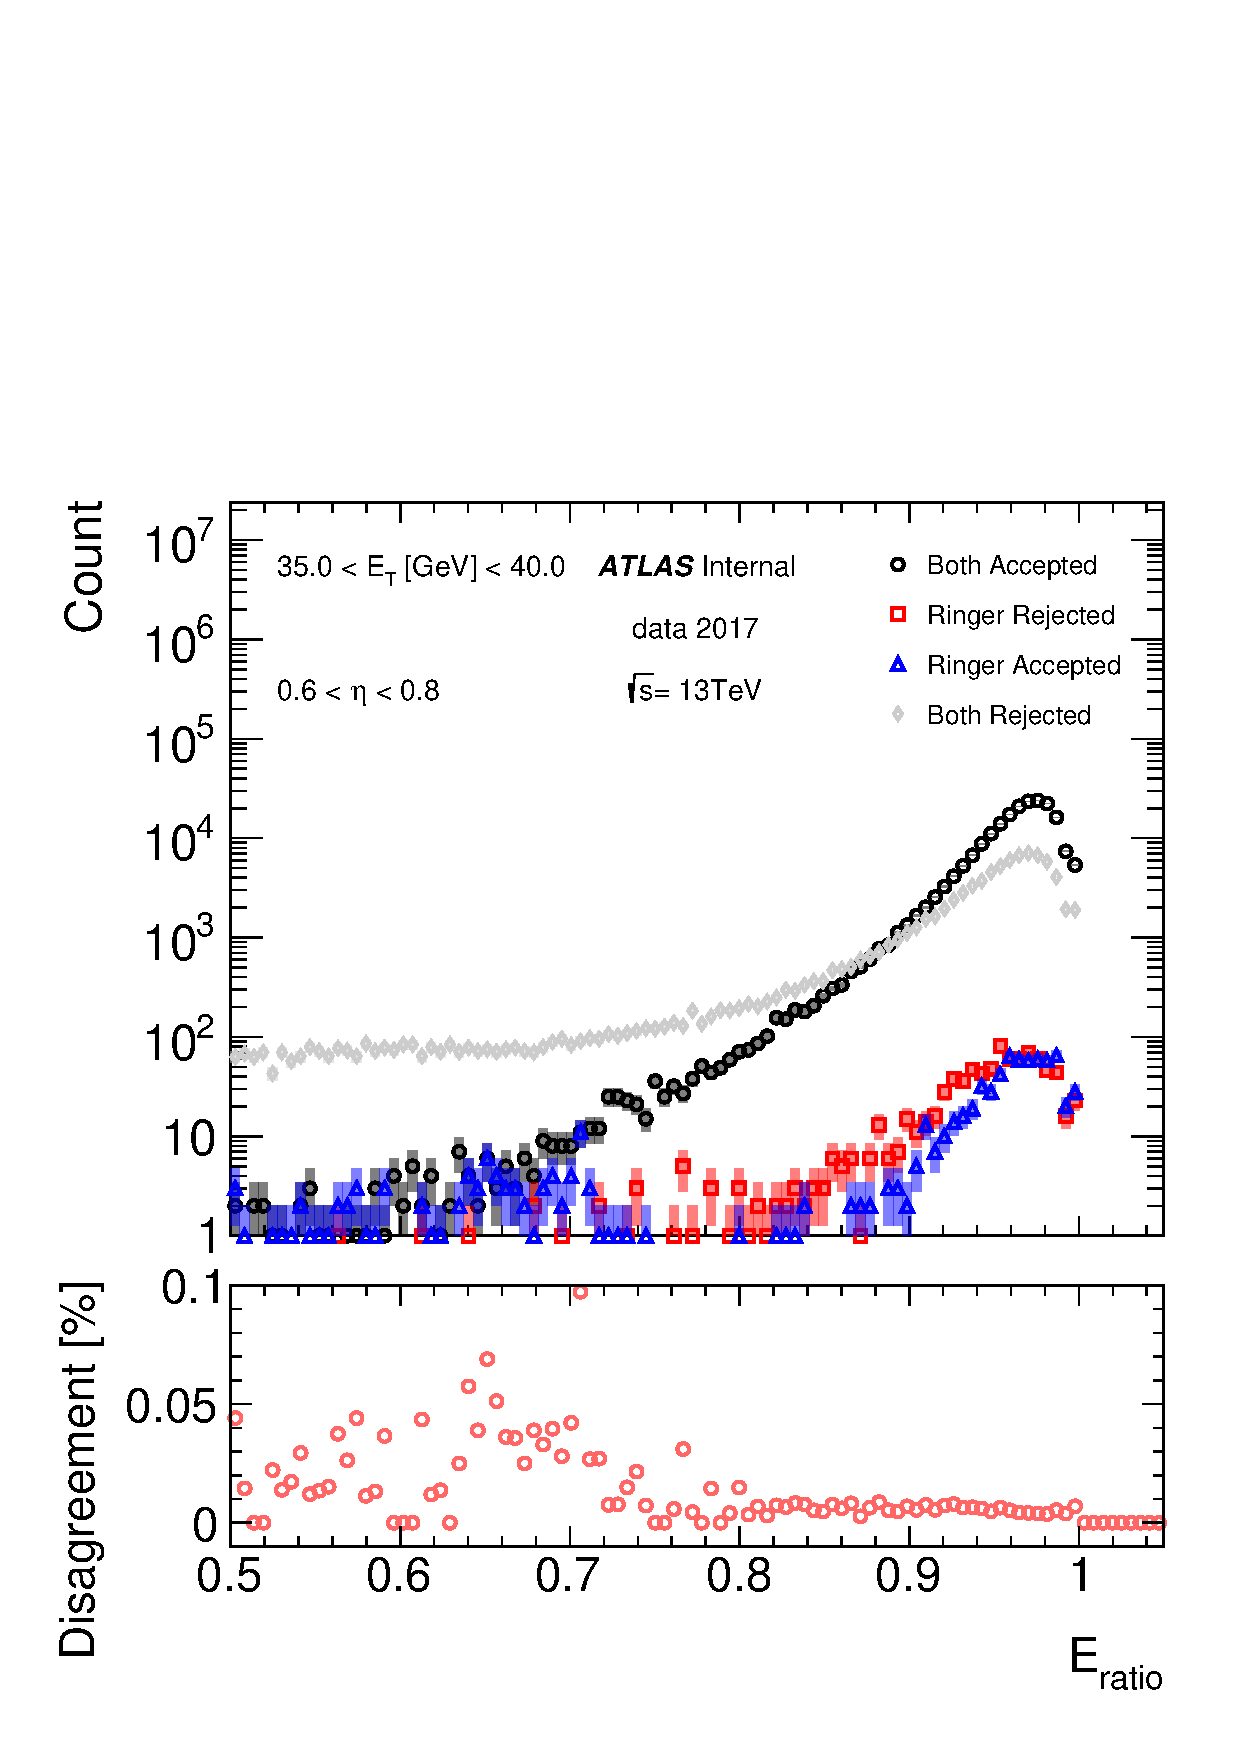
\includegraphics[width=\textwidth]{sections/04_analysis/figures/quadrant_plots/eratio.pdf}
\caption{}
\end{subfigure}
\hfill
\begin{subfigure}[c]{.49\textwidth}
\centering
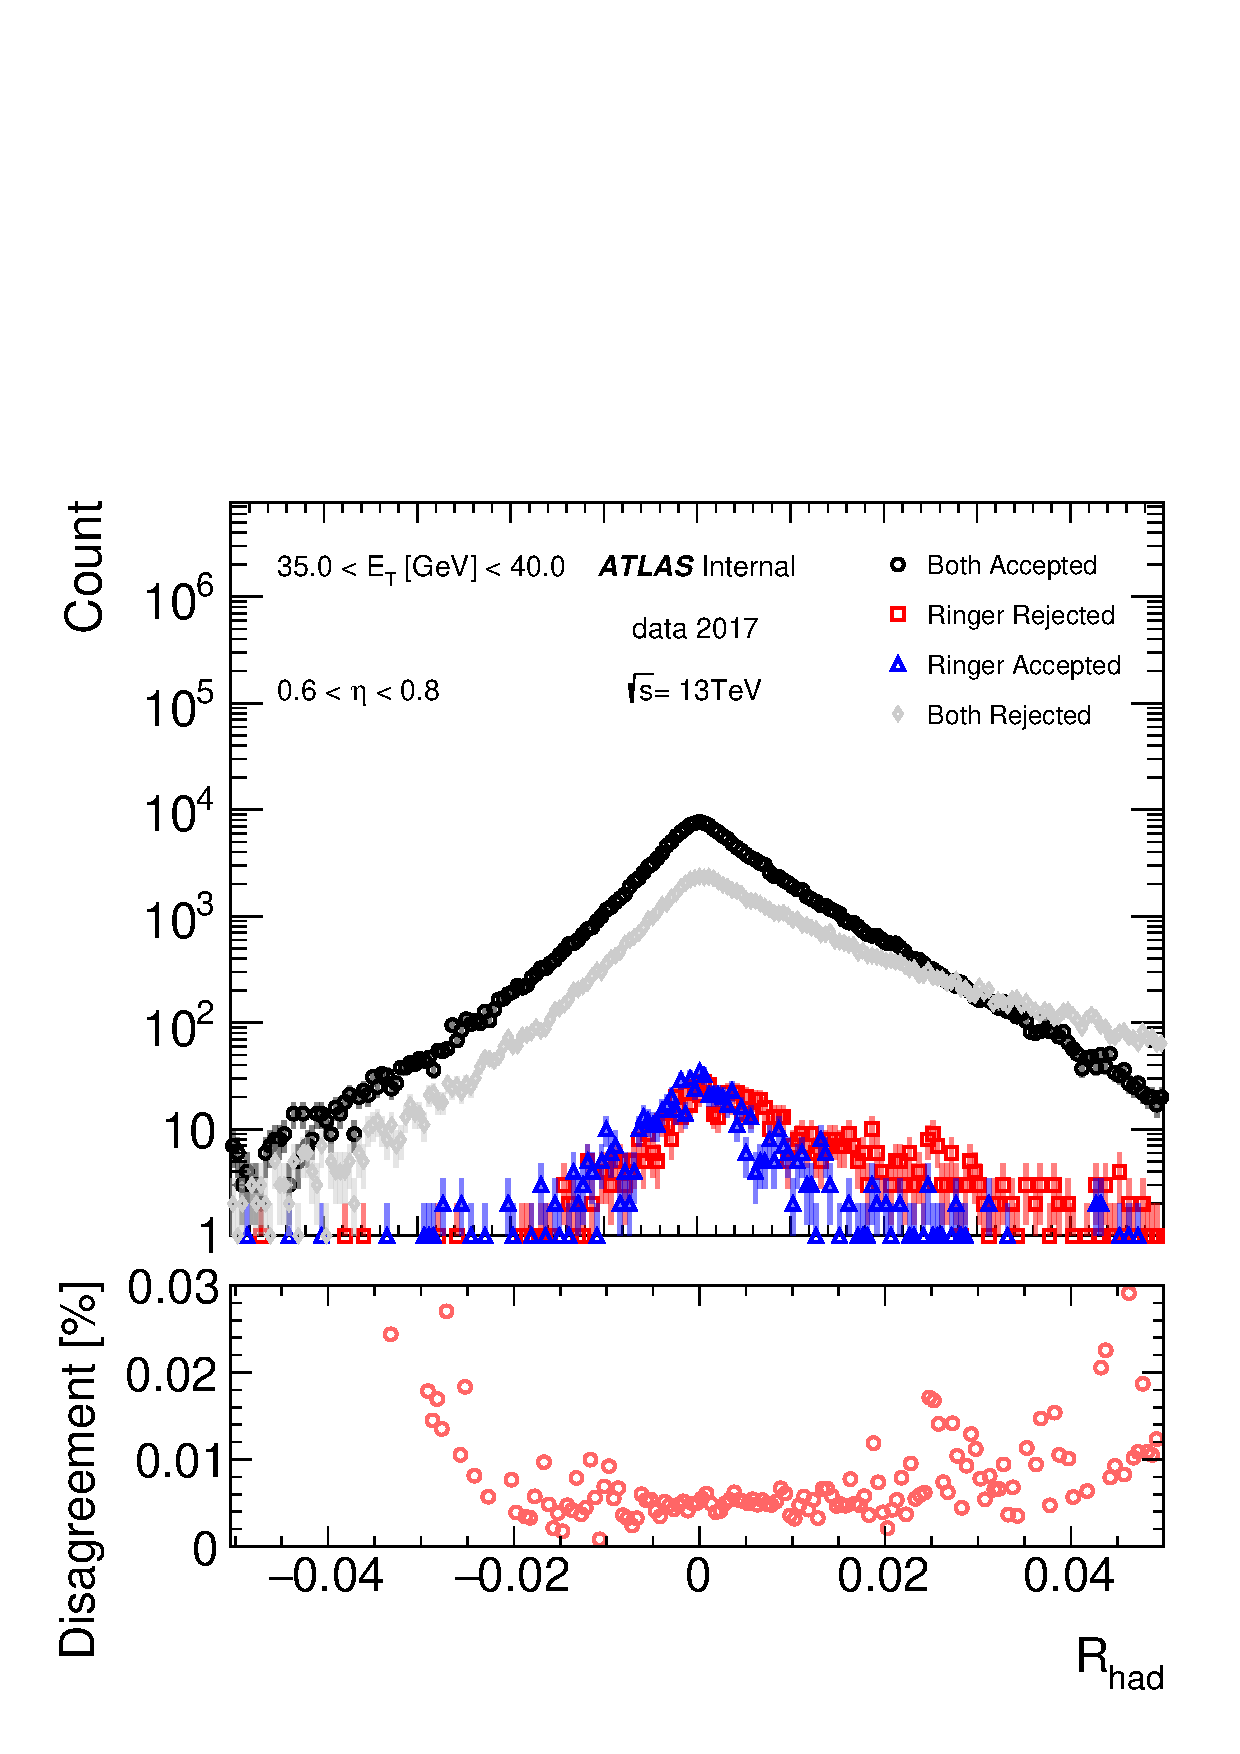
\includegraphics[width=\textwidth]{sections/04_analysis/figures/quadrant_plots/rhad.pdf}
\caption{}
\end{subfigure} \\


\caption{\label{fig:quadrant_calo_variables_30GeV}
	Quadrant analysis plots for the main offline-reconstructed
	calorimetry variables employed in the
	likelihood and for the $0.6<\abseta{}<0.8$ and
	$30<\et{}~[\text{GeV}]<35$ slices. 
	The top pad in each figure shows the raw number of observations for the four mutually exclusive cases: both with and without \rnn{}
	triggered (black); triggered only with \rnn{} (blue); triggered only without \rnn{} (red); neither one triggered (gray). The bottom pad contains disagreement as defined in the Equation \eqref{eq:disagreement}.
}
%Quadrant analysis plots for the offline-reconstructed
%calorimetry variables employed in the
%likelihood and \wstot{} for the $0.6<\abseta{}<0.8$ and
%$30<\et{}~[\text{GeV}]<40$ slices.}%
\end{figure}

Although similar behavior is shown for the other 
regions, the differences vary in strength in each \abseta{} region. As expected, 
the trigger does not show a dependence on ID variables, as shown in Figure~\ref{fig:quadrant_track_variables_30GeV} for $35<\et{}~[\text{GeV}]<40$, since the only distinction between them is the electron identification model operating in the \fastcalo{}.


\begin{comment}
    
\begin{figure}[h!tb]
%\centering
%\begin{subfigure}[c]{.49\textwidth}
\centering
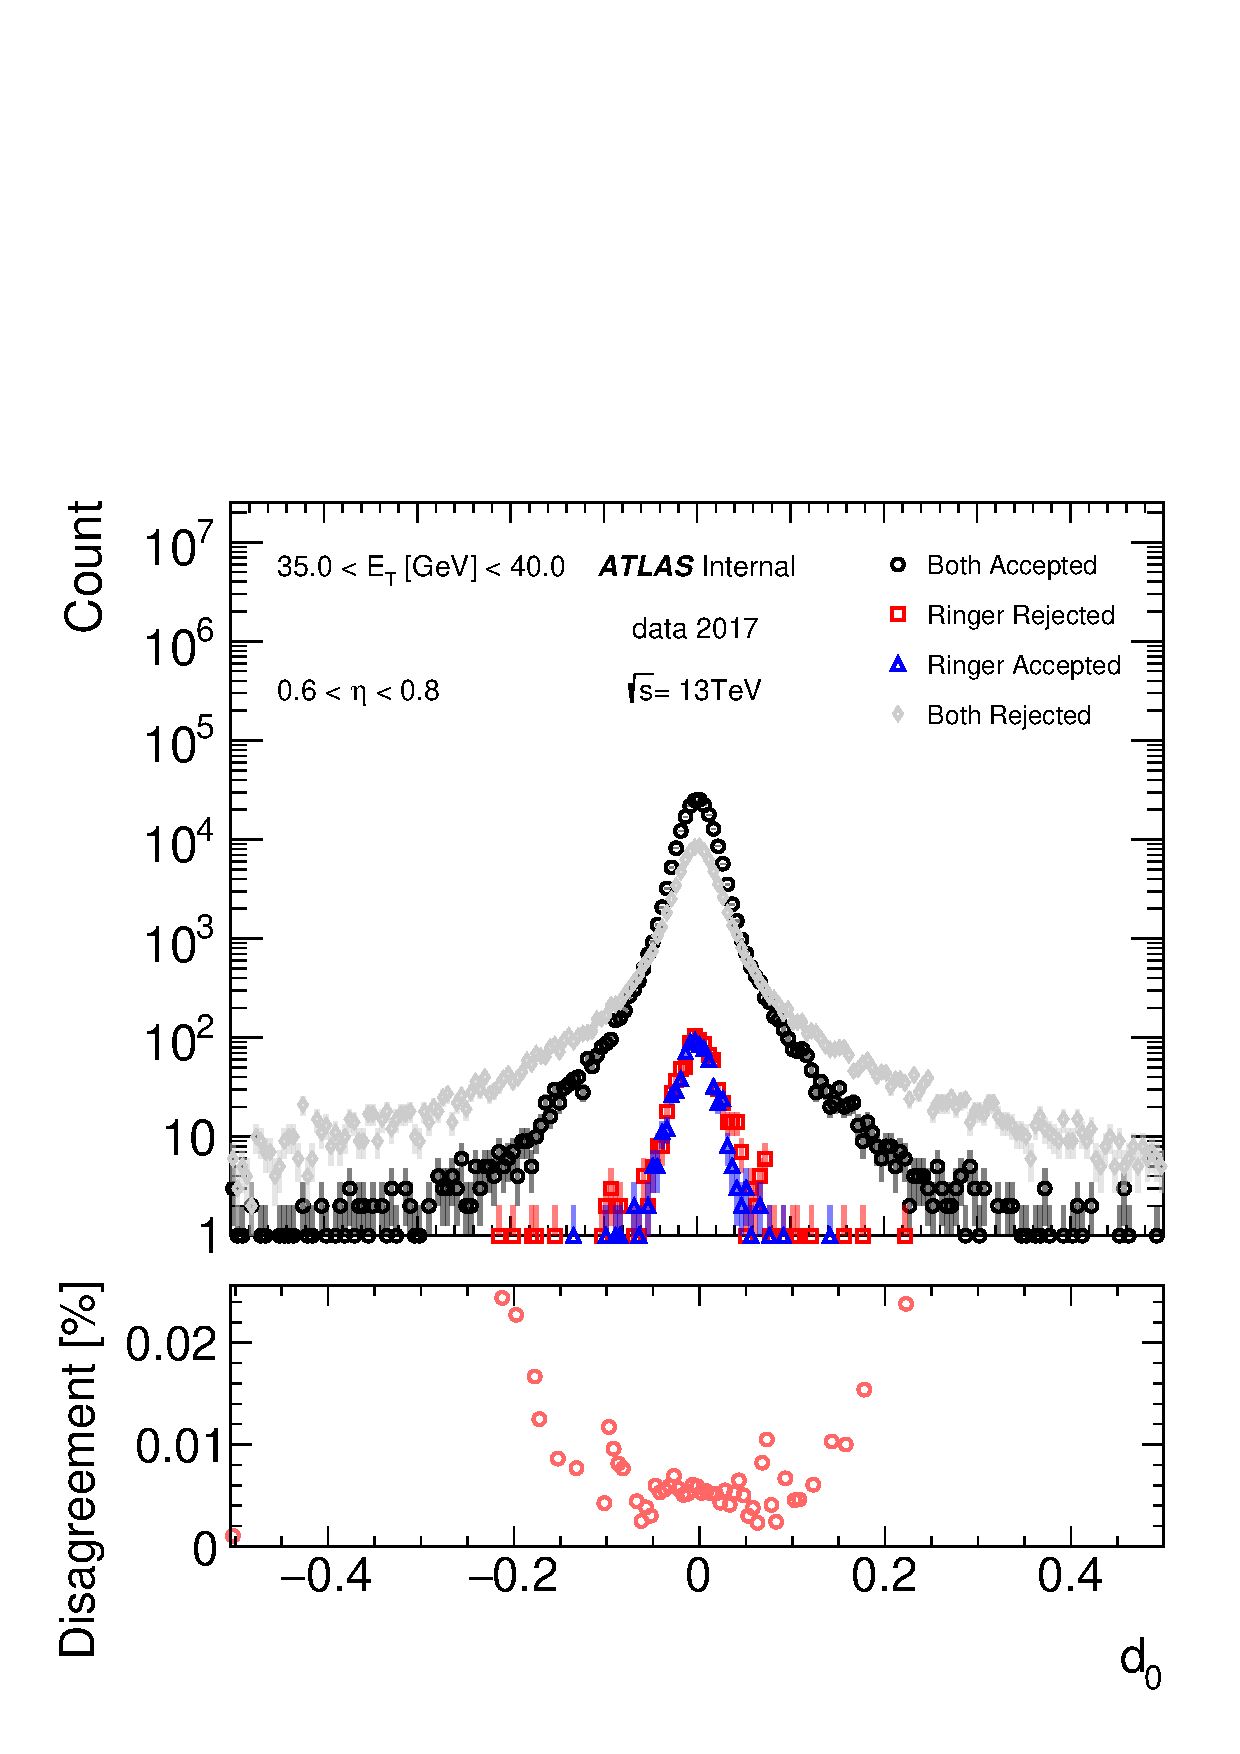
\includegraphics[width=.5\textwidth]{sections/04_analysis/figures/quadrant_plots/d0.pdf}
\caption{\label{fig:quadrant_track_variables_30GeV}
Quadrant analyses plots for the offline-reconstructed ID variable $d_0$ employed in the
likelihood for the $0.6<\abseta{}<0.8$ and $35<\et{}~[\text{GeV}]<40$ slice. The variable $d_0$ is defined as the transverse parameter of the impact point with respect to the collision beam.
}
\end{figure}
\end{comment}






\FloatBarrier
\subsection[Homogeneity Tests]{Homogeneity Tests}\label{ssec:agreement}

In this 
analysis, the impact of using different triggers, \rnn{} and cut-based, on the likelihood algorithm is evaluated. This study requires a pair of duplicated triggers, composed by an $E_T > 28$ GeV isolated and Tight selection with and without the \rnn{}, operating online together. 
This analysis is performed using \Zee{} \tnp{} collision data, which were selected with the trigger requirement set to either one of the duplicated triggers for the tag, whereas the probe selection is invariably set to the offline \vloose{} criterion. This is the exact setup employed by ATLAS to derive the offline likelihood for electrons above \SI{15}{\GeV}~\cite{aaboud2019electron}. To benefit from the full 2017 statistics, collision data collected previous to the TS1 were also employed. In case the profiles are statistically identical, then it is expected that the \rnn{} trigger does not cause any relevant alteration in the derivation of the offline likelihood pdfs.  The statistical method for profile evaluation is described in Section~\ref{top:homogeneity_method} and the results are available in Section~\ref{top:agreement_homogeneity_results}.




\subsubsection{Method}\label{top:homogeneity_method}



The problem is approached based on homogeneity tests on histograms~\cite{homogeneity_test}, in order to check for (systematic) effects of the trigger configuration. It is based on a test originally developed by Pearson~\cite{pearson1911probability} and popularly employed in many fields beyond High Energy Physics (HEP), e.g. social sciences~\cite{wickens2014multiway} and health~\cite{ma2015homogeneity}, usually labelled as contingency or consistency tests.

In order to benefit from the test without having to customize it to the ATLAS particular analysis setup, the collision data was split into two
statistically independent groups attempting to keep data taking conditions as
similar as possible by successively taking data to each group from small
consecutive periods. 

By comparing the p-values of the two groups, it is possible to evaluate how the different configuration affects the likelihood of the profiles to be drawn from the same distribution. If the p-values\footnote{The p-value here is defined by: $P-value \approx f(x, k) = \frac{1}{2^{k/2}\Gamma(k/2)}x^{k/2 -1}e^{-x/2}$} have negligible fluctuations with respect to the values obtained by the tests comparing the same triggers, then the systematic effect in the profiles is negligible with respect to half\footnote{Once each group is using nearly half of the integrated luminosity.} of the statistics available.



To provide a better insight on possible distortions, the corresponding $\chi$
individual contributions of each group are computed allowing them to freely
oscillate through the positive and negative axis with

\begin{equation}
  \chi_{i,j}^{s} = \frac{(r_{i,j} - b_{i,j})}{\sqrt{b_{i,j}}},
  \label{eq:signed_chi}
\end{equation}

\noindent where $r_{i,j}$ ($b_{i,j}$) is the number of observations collected by
the trigger with (without) \rnn{} in $j$th histogram bin and in the $i$th
$\et{}\times\abseta{}$ region.


\subsubsection{Results}\label{top:agreement_homogeneity_results}




Regardless of the trigger configuration, the p-values of the homogeneity tests between the two groups result in similar values. In other words, the fluctuations in the profiles are mainly dominated by statistical fluctuations, with no sign of systematic effects due to the trigger configuration. 

Similar behavior is observed for the ID and calo-ID variables. The Figure~\ref{fig:groups_homogeneity_calo} shows the residuals when considering the histogram obtained with collision data collected by the trigger without \rnn{} for the first arbitrary group as a reference. The residuals are dominated by statistical fluctuations, which are within the expectations from homogeneity hypothesis for most variables and regions.


\begin{figure}[b]
\begin{center}
\begin{subfigure}[c]{.48\textwidth}
\centering
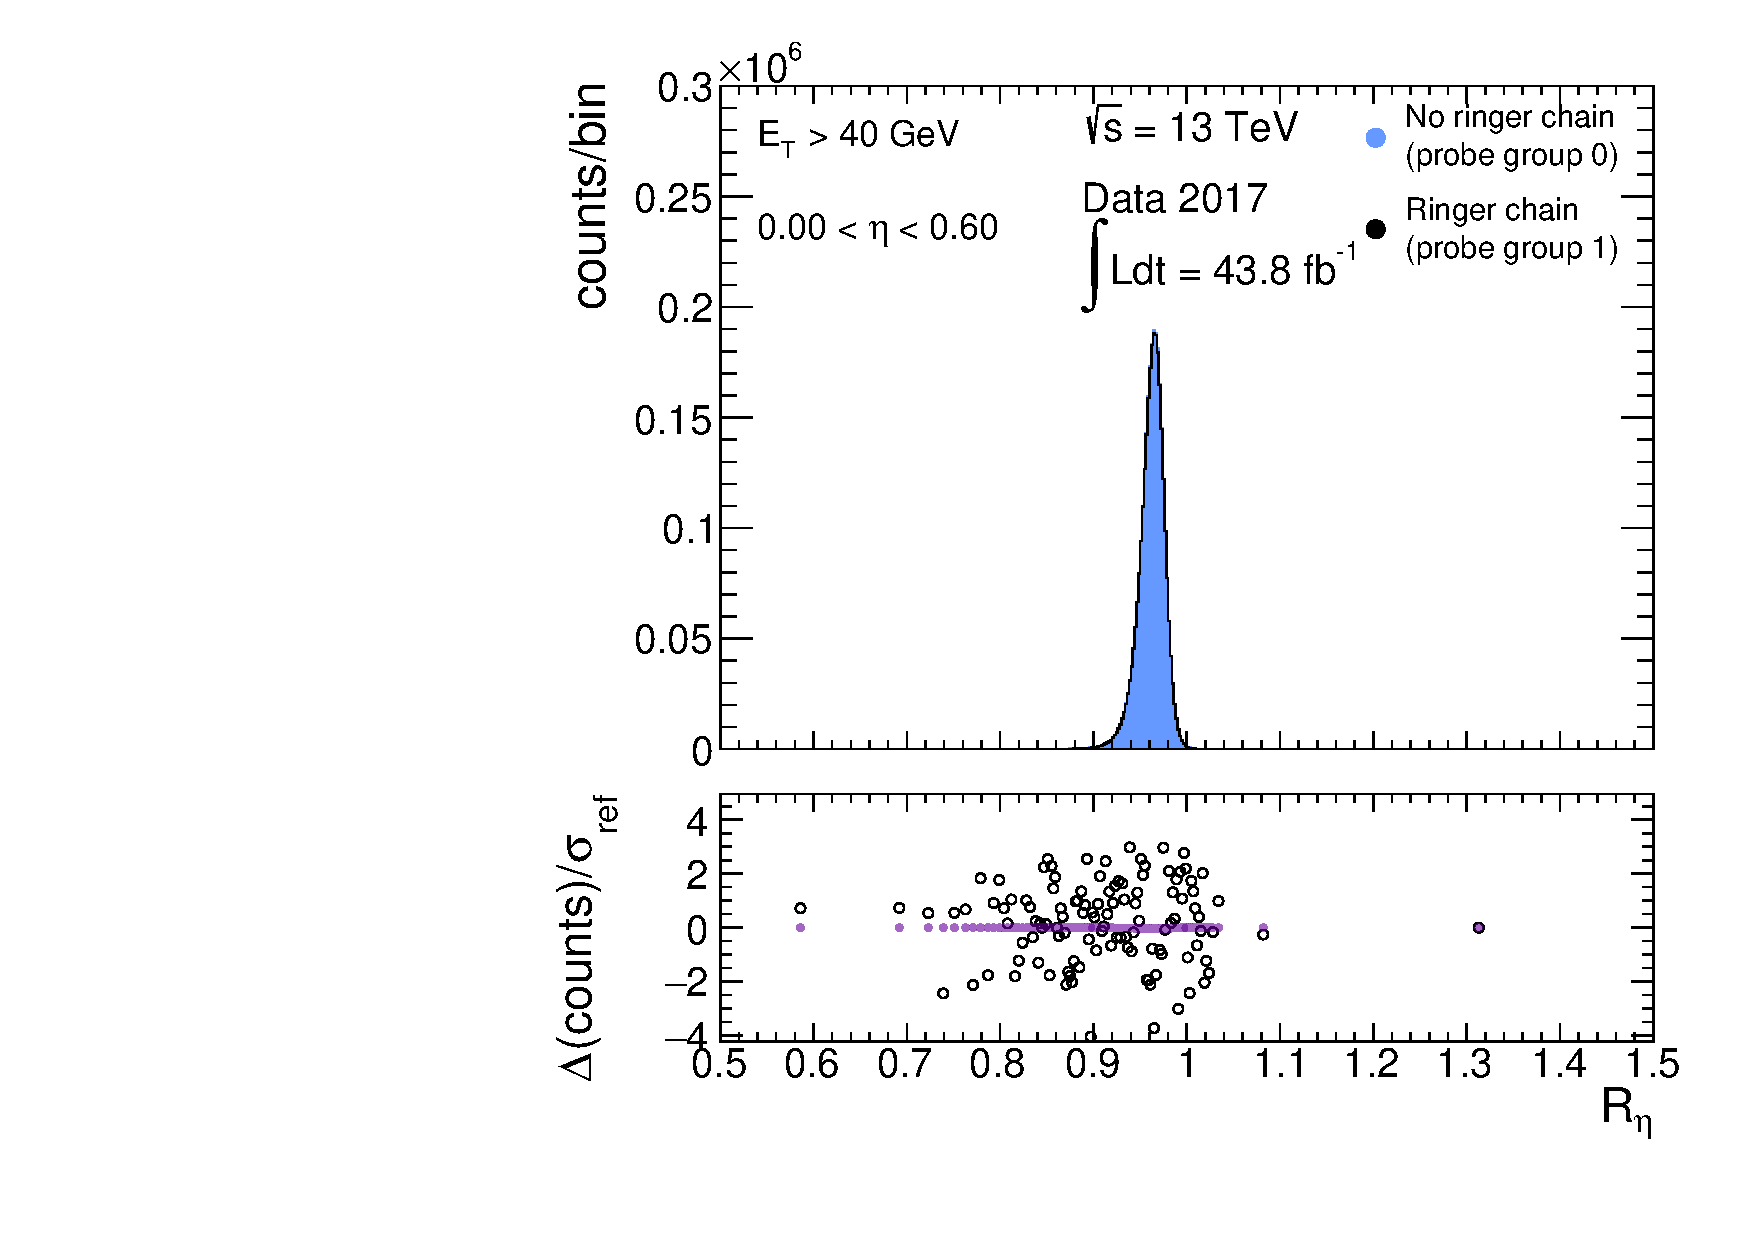
\includegraphics[width=\textwidth]{sections/04_analysis/figures/noAdjustment/el_reta_et40eta0_00_sigma_base_new.pdf}
\caption{}%

\end{subfigure}
\hfill
\begin{subfigure}[c]{.48\textwidth}
\centering
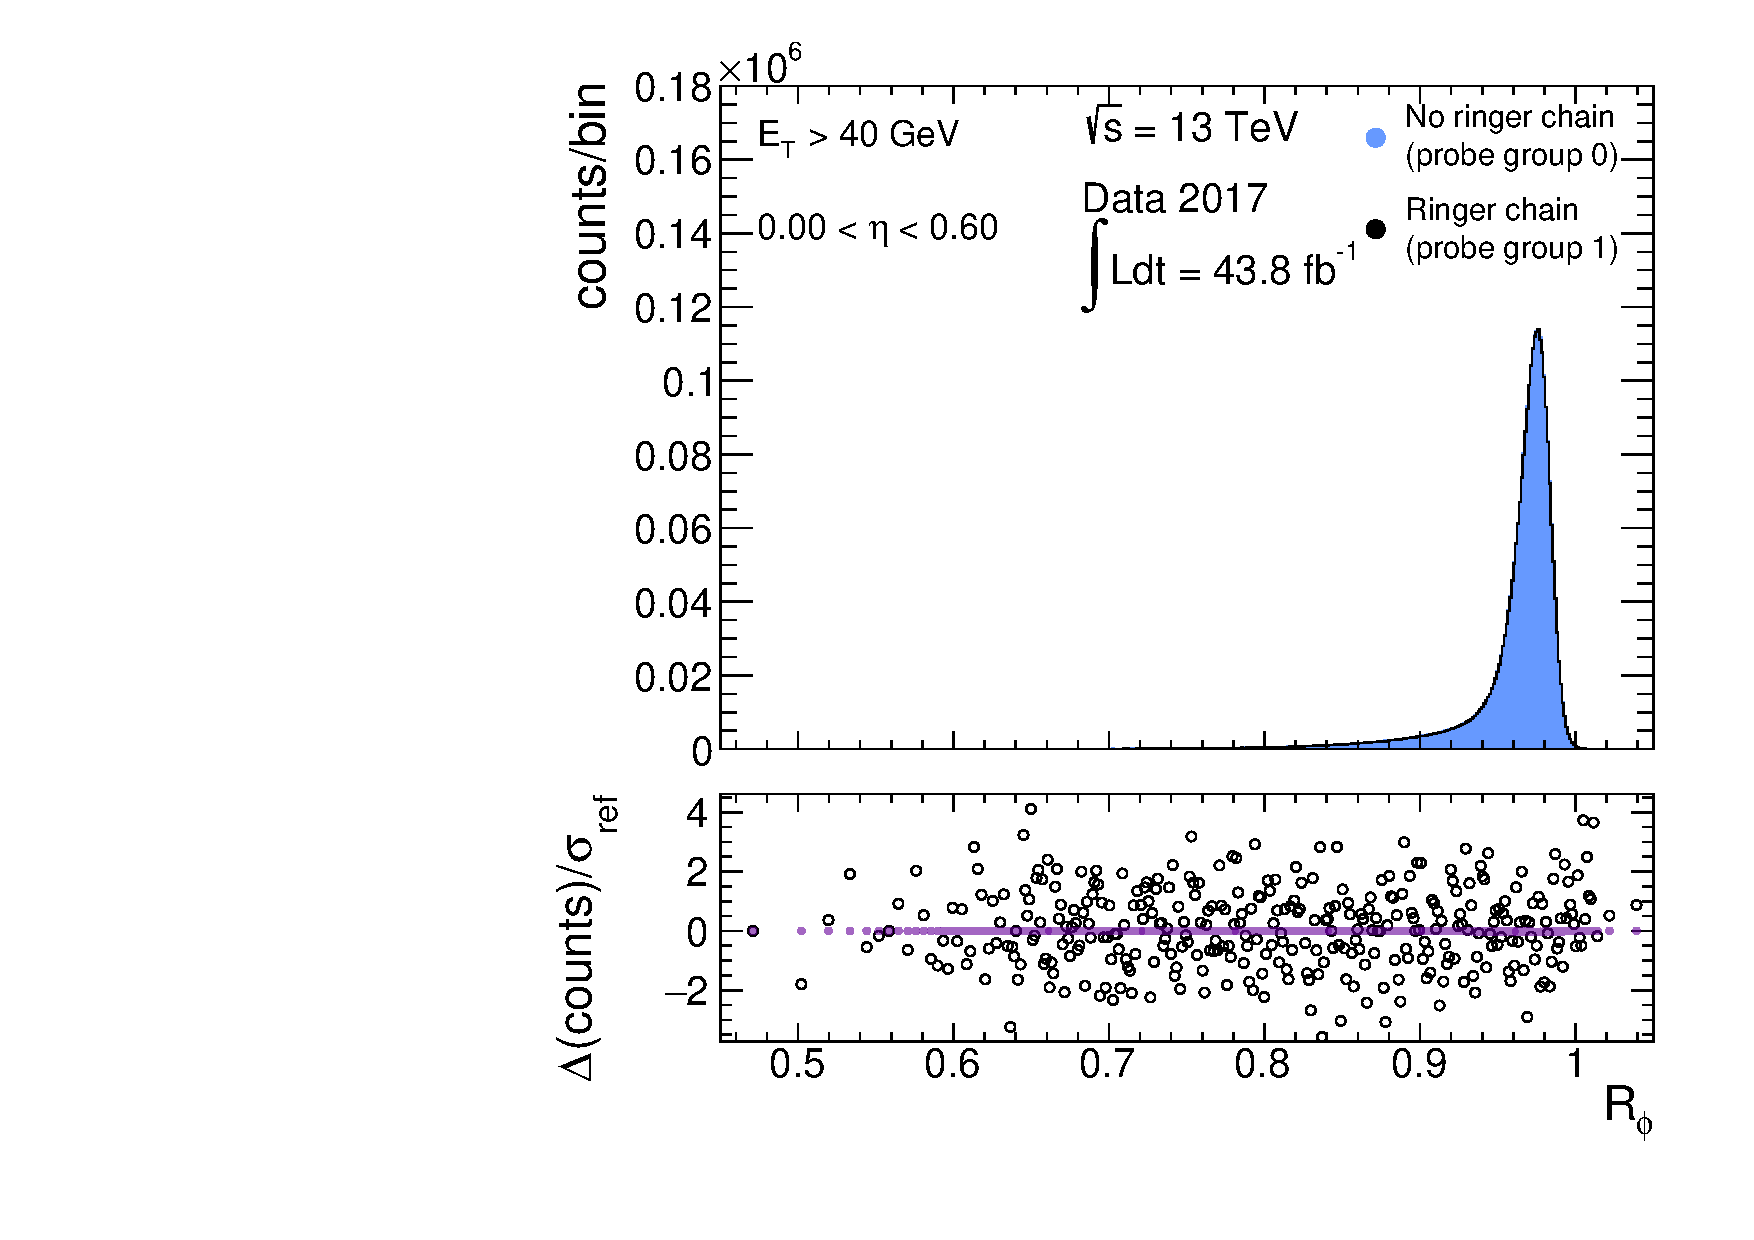
\includegraphics[width=\textwidth]{sections/04_analysis/figures/noAdjustment/el_rphi_et40eta0_00_sigma_base_new.pdf}
\caption{}%

\end{subfigure} \\
\begin{subfigure}[c]{.48\textwidth}
\centering
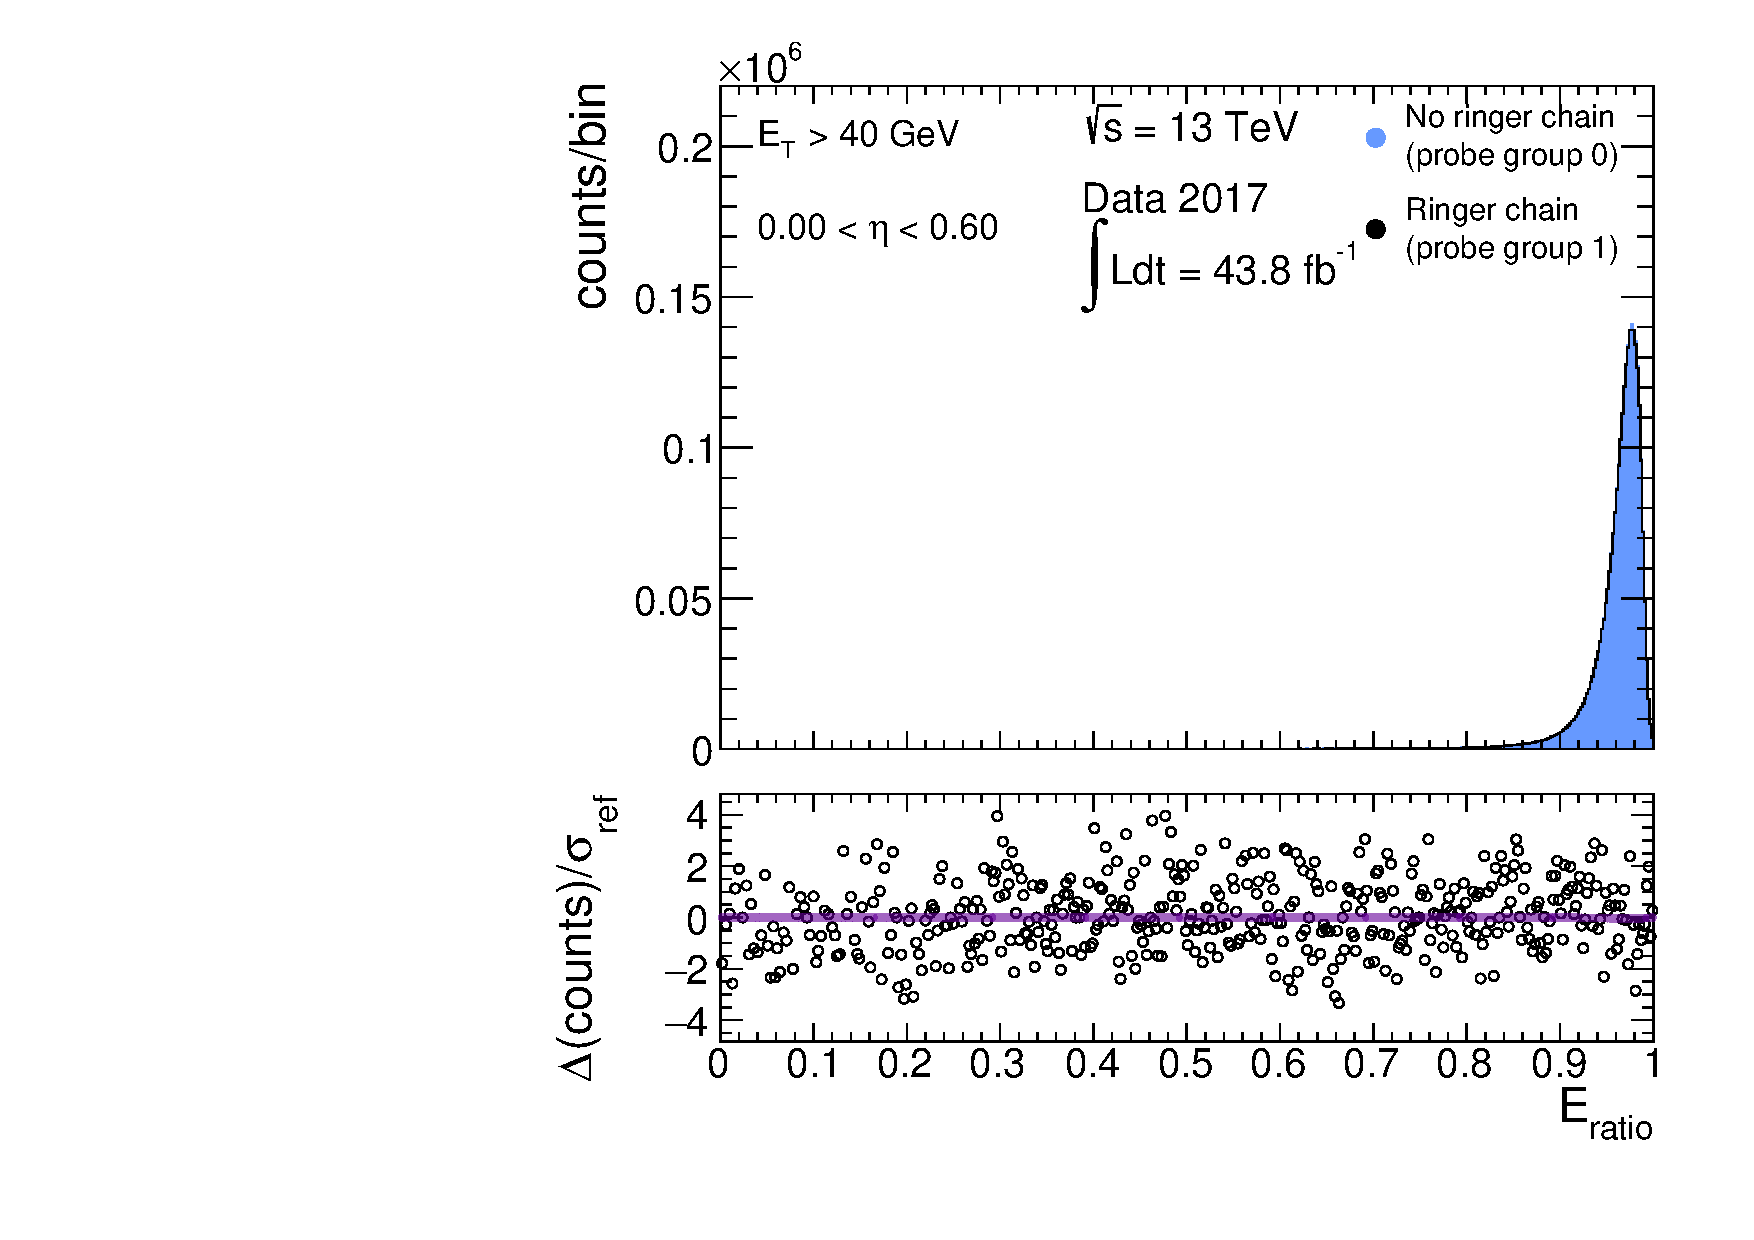
\includegraphics[width=\textwidth]{sections/04_analysis/figures/noAdjustment/el_eratio_et40eta0_00_sigma_base_new.pdf}
\caption{}%

\end{subfigure}
\hfill
\begin{subfigure}[c]{.48\textwidth}
\centering
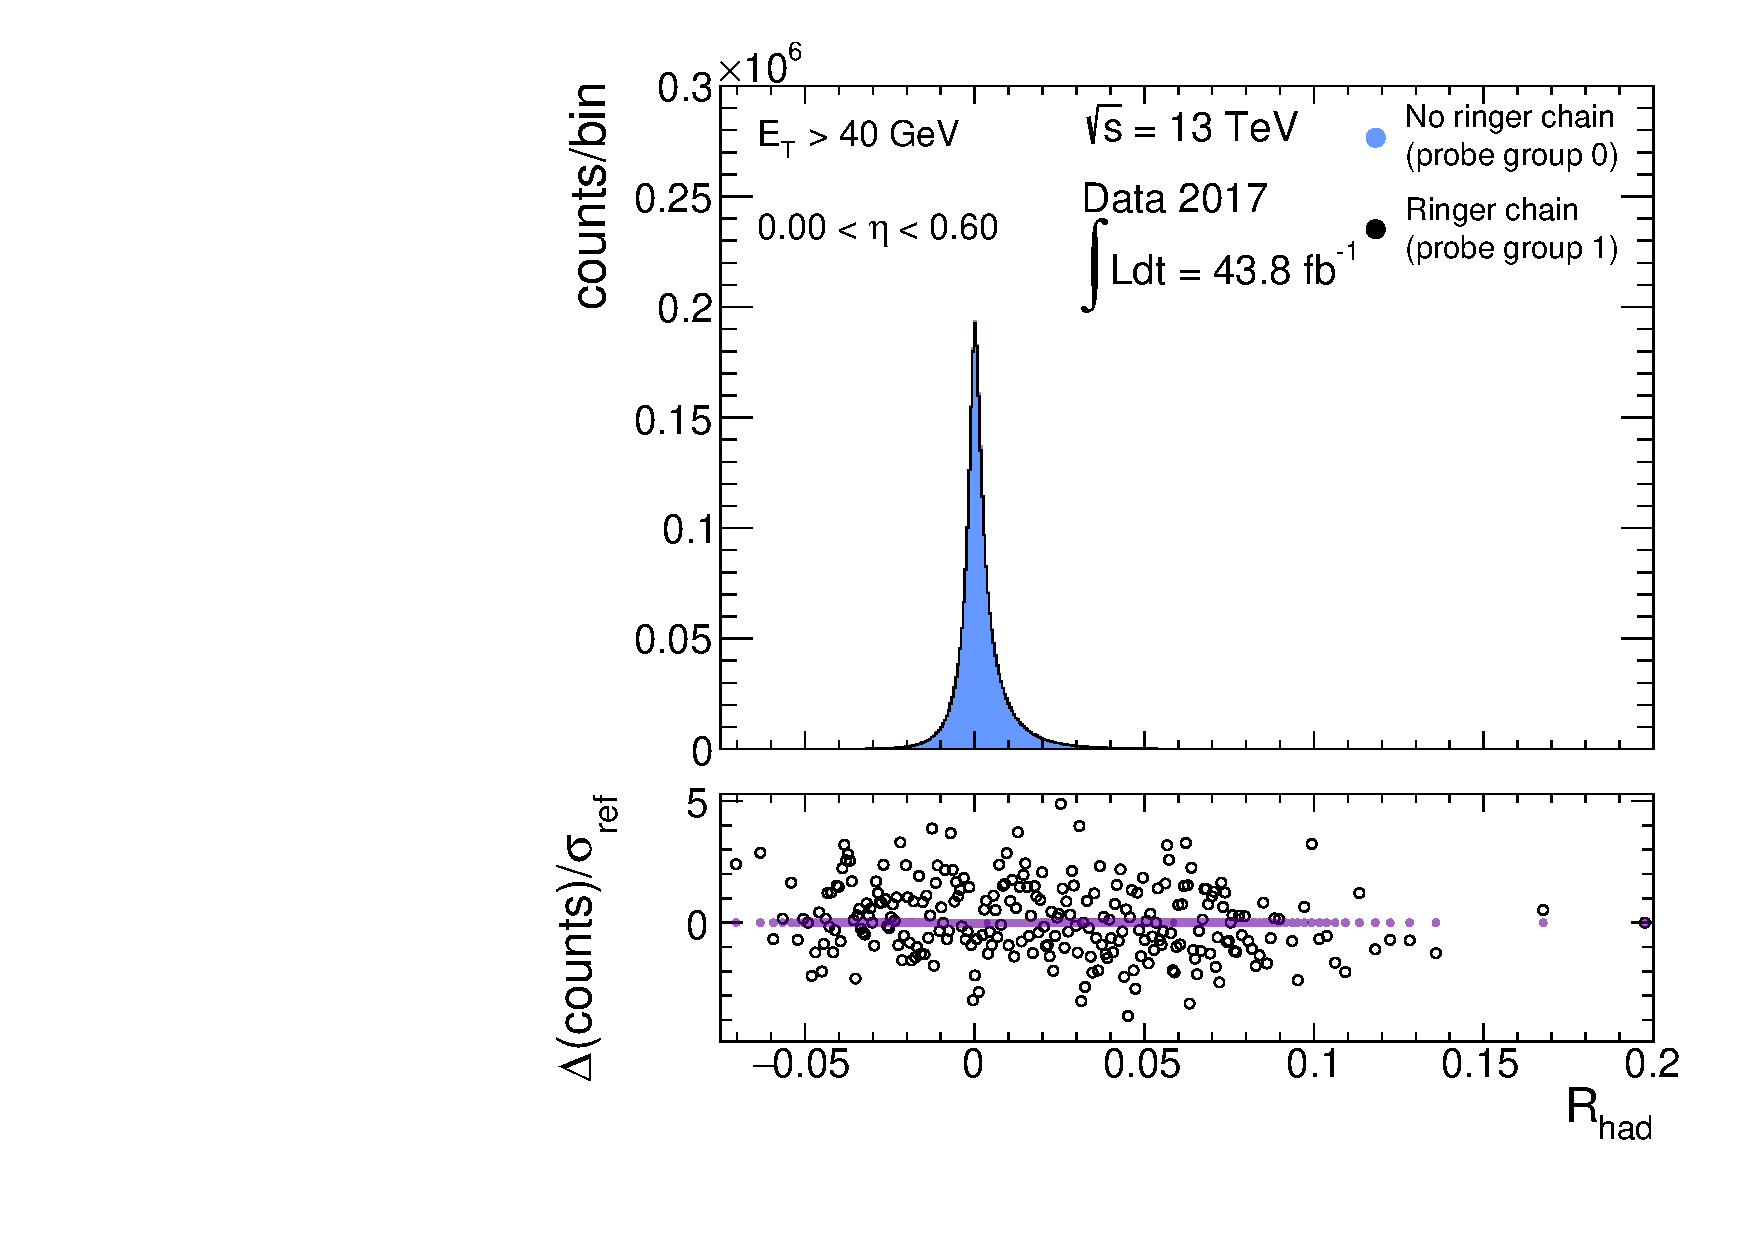
\includegraphics[width=\textwidth]{sections/04_analysis/figures/noAdjustment/el_rhad_et40eta0_00_sigma_base_new.pdf}
\caption{}%

\end{subfigure} \\
\caption{%
	Top: \reta, \eratio, \rphi, \rhad histogram profiles for the calorimetry variables employed in the offline likelihood in the $\et>\SI{40}{\GeV}$ and $0.00<\abseta{}<0.80$ regions using collision data collected by
	triggering without \rnn{} in the first arbitrary data group
	(blue area) and collision data collected by triggering with \rnn{} in the second
	arbitrary data group (black line).  Bottom: residual contributions using as
	statistics $\chi^s$ (equation~\ref{eq:signed_chi}, in black) and the expected
	model for no distortion given by the $\chi^s$ residuals w.r.t.\@ the
	reference.
}%
\label{fig:groups_homogeneity_calo}
\end{center}
\end{figure}%


\FloatBarrier
